%% -*- coding:utf-8 -*-
\documentclass[10pt,pdf,hyperref={unicode}]{beamer}
\input ./preamble.tex
\usetheme{Warsaw}
\title[Криптография и квантовые вычисления]{Классическая
  криптография\\Квантовые вычисления}
\author{Мурашко И. В.}
\institute{Санкт Петербургский Государственный Политехнический Университет}
\date{}
\begin{document}

\begin{frame}
\titlepage
\end{frame}


\section{Введение}

\begin{frame}{Введение}
\begin{itemize}
\item Квантовая механика
\item Квантовые вычисления
\item Методы симметричного шифрования и алгоритм Гровера
\item Методы несимметричного шифрования (RSA, Diffie-Hellman, Elliptic
curve) и алгоритм Шора.
\end{itemize}
\end{frame}

\section{Квантовая механика}
\begin{frame}{Двухуровневый атом}
\begin{figure}
\centering

\input ../add/quant/picmeasurex.tex

\caption{Процесс измерения энергии двухуровневого атома находящегося в
чистом состоянии $\left|\psi\right> = 
\frac{1}{\sqrt{2}}\left|a\right> + \frac{1}{\sqrt{2}}\left|b\right>$.
Прибором регистрируется значение энергии $E_a$ или $E_b$.
}
\label{fig:add:mesure_ex}
\end{figure}
\end{frame}

\begin{frame}{Двухуровневый атом. Измерение $E_a$}
\begin{figure}
\centering

\input ../add/quant/picmeasurex_a.tex

\caption{Процесс измерения энергии двухуровневого атома находящегося в
чистом состоянии $\left|\psi\right> = 
\frac{1}{\sqrt{2}}\left|a\right> + \frac{1}{\sqrt{2}}\left|b\right>$.
Прибором регистрируется значение энергии $E_a$. При измерении
происходит следующая редукция $\left|\psi\right> \to \left|a\right>$
}
\label{fig:add:mesure_ex_a}
\end{figure}
\end{frame}

\begin{frame}{Двухуровневый атом. Измерение $E_b$}
\begin{figure}
\centering

\input ../add/quant/picmeasurex_b.tex

\caption{Процесс измерения энергии двухуровневого атома находящегося в
чистом состоянии $\left|\psi\right> = 
\frac{1}{\sqrt{2}}\left|a\right> + \frac{1}{\sqrt{2}}\left|b\right>$.
Прибором регистрируется значение энергии $E_b$. При измерении
происходит следующая редукция $\left|\psi\right> \to \left|b\right>$
}
\label{fig:add:mesure_ex_b}
\end{figure}
\end{frame}

\begin{frame}{Кот Шредингера}
 \begin{figure} 
   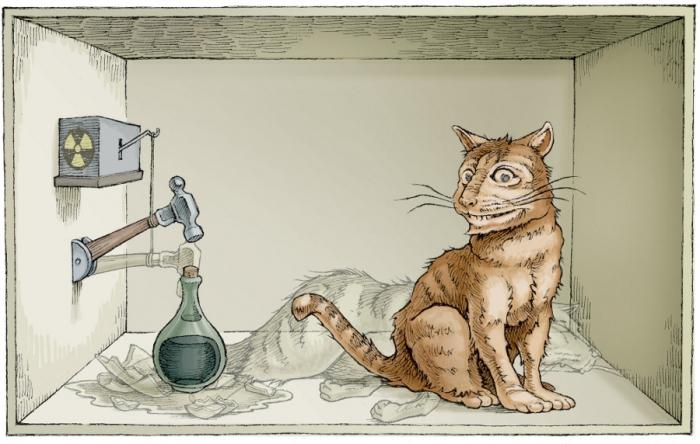
\includegraphics[width=90mm,scale=0.5]{catshred.jpg}
  \end{figure}
\end{frame}

\begin{frame}{Эксперимент Белла. Классический случай}
\[
f = \frac{1}{2}\left(
a b + a' b + a b' - a' b'
\right), a,a',b,b' \in \{-1, +1\}.
\]
следовательно
\(
f \in \{-1, +1\}
\)
и
\(
\left|\left<f\right>\right| \le 1
\)
\end{frame}

\begin{frame}{Эксперимент Белла. Квантовый случай}
\[
\left|\left<f\right>\right| = \sqrt{2} > 1
\]
\end{frame}


\begin{frame}{Отрицательные вероятности}
\[
\left<f\right> = \sum_{a,a',b,b'} p(a,a',b,b') f(a,a',b,b').
\]
следовательно для $\left|\left<f\right>\right| > 1$ необходимо
\[
\exists a,a',b,b': p(a,a',b,b') < 0
\]
\end{frame}

\section{Квантовые вычисления}
\begin{frame}{Классические вычисления}
\begin{figure}
\centering

\input ../part4/quantcomp/picclasscomp.tex

\caption{Классические вычисления. На вход подается число $x$ состоящее
  из $n$ бит, а на выходе имеем результат $y = f\left(x\right)$ описываемый $m$ битами}
\label{figQuantCompClassComp}
\end{figure}
\end{frame}

\begin{frame}{Квантовые вычисления}
\begin{figure}
\centering

\input ../part4/quantcomp/picquantcomp.tex

\caption{Квантовые обратимые вычисления. На вход подается число
  $\left|x\right>$ состоящее из $n$ кубит и затравка из нулевых
  состояний ($m$ кубит), а на выходе имеем результат $\left|y\right> =
  \left|f\left(x\right)\right>$ описываемый $m$ кубитами и исходное
  состояние $\left|x\right>$} 
\label{figQuantCompQuantComp}
\end{figure}
\end{frame}


\begin{frame}{Квантовые вычисления}
Классический случай
\[
x \to f(x)
\]
Квантовый случай
\begin{eqnarray}
\left|0\right>\left|0\right> + \left|1\right>\left|0\right> + \left|2\right>\left|0\right> +
\dots + \left|x\right>\left|0\right> + \dots \to
\nonumber \\
\to 
\left|0\right>\left|f(0)\right> + \left|1\right>\left|f(1)\right> + \left|2\right>\left|f(2)\right> +
\dots + \left|x\right>\left|f(x)\right> + \dots
\nonumber
\end{eqnarray}
\end{frame}


\section{Алгоритм Гровера}
\begin{frame}{Задача о поиске иголки в стоге сена}
\begin{figure}
\centering

\input ../part4/quantcomp/picsearch.tex

\caption{Поиск в неструктурированном объеме данных (поиск "иголки в
  стоге сена"). Классическая сложность $O(N)$}
\label{figQuantCompSearch}
\end{figure}
\end{frame}

\begin{frame}{Алгоритм Гровера. Схема}
\begin{figure}
\centering

\input ../part4/quantcomp/picgrover.tex

\caption{Алгоритм Гровера. Сложность $ O(\sqrt{N})$}
\label{figQuantCompGrover}
\end{figure}
\end{frame}

\begin{frame}{Алгоритм Гровера. Схема}
\begin{figure}
\centering

\input ../part4/quantcomp/picgroverbase.tex

\caption{Алгоритм Гровера}
\label{figQuantCompGrover}
\end{figure}
\end{frame}


\begin{frame}{Алгоритм Гровера. Принцип работы}
\begin{figure}
\centering

\input ../part4/quantcomp/picgroverinv.tex

\caption{Алгоритм Гровера. Инверсия фазы}
\label{figQuantCompGroverInv}
\end{figure}
\end{frame}

\begin{frame}{Алгоритм Гровера. Принцип работы}
\begin{figure}
\centering

\input ../part4/quantcomp/picgroverinvmiddle.tex

\caption{Алгоритм Гровера. Обращение относительно
  среднего.}
\label{figQuantCompGroverInvMiddle}
\end{figure}

\end{frame}


\begin{frame}{Влияние на рекомендации к использованию}
$O(N) \rightarrow O(\sqrt{N})$
ведет например к следующей рекомендации
$AES_{128} \rightarrow AES_{256}$
\end{frame}


\section{Алгоритм Шора}
\begin{frame}{RSA и задача факторизации чисел}
TBD
\end{frame}

\begin{frame}{Diffie-Hellman, Elliptic
curve и дискретный логарифм}
TBD
\end{frame}

\begin{frame}{Задача о нахождении периода функций и алгоритм Шора}
TBD
\end{frame}

\begin{frame}{Влияние на рекомендации к использованию}
NSA не рекомендует использование алгоритмов на элиптических кривых для
внутреннего использования.
\end{frame}

\section{Заключение}
\begin{frame}{Что дальше?}
TBD
\end{frame}

\begin{frame}{Вопросы}
TBD
\end{frame}

\end{document}
